\documentclass[border=10pt]{standalone}
\usepackage{tikz}
\usetikzlibrary{shapes.multipart,arrows.meta,calc}
\definecolor{cwork}{RGB}{72,116,158}
\definecolor{cpm}{RGB}{222,158,74}
\begin{document}
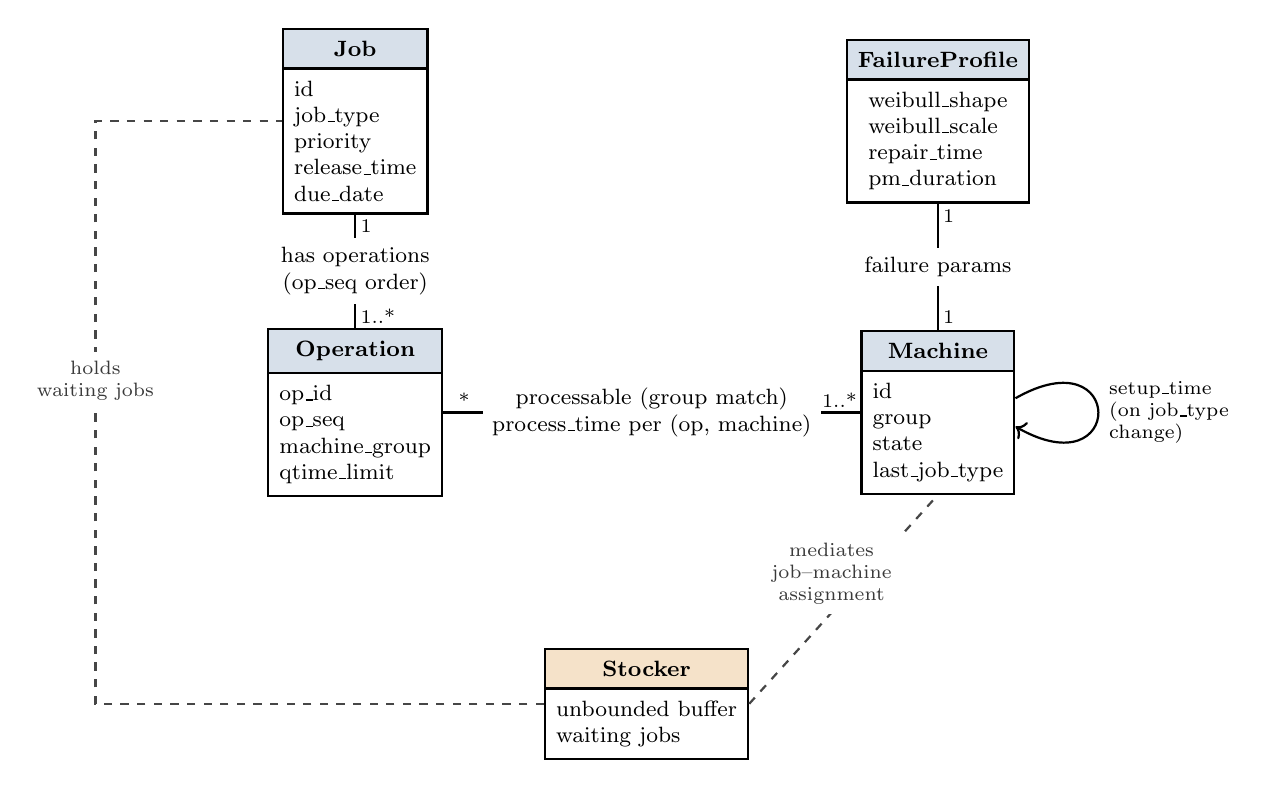
\begin{tikzpicture}[font=\footnotesize,
   entity/.style={rectangle split, rectangle split parts=2, draw, thick,
     rectangle split part fill={cwork!22,white}, align=left, inner sep=4pt},
   rel/.style={thick}, mult/.style={font=\scriptsize,inner sep=1.5pt}]
  \node[entity] (job) at (0,3.7)
    {\textbf{Job}\nodepart{two}id\\job\_type\\priority\\release\_time\\due\_date};
  \node[entity] (op) at (0,0)
    {\textbf{Operation}\nodepart{two}op\_id\\op\_seq\\machine\_group\\qtime\_limit};
  \node[entity] (mc) at (7.4,0)
    {\textbf{Machine}\nodepart{two}id\\group\\state\\last\_job\_type};
  \node[entity] (fp) at (7.4,3.7)
    {\textbf{FailureProfile}\nodepart{two}weibull\_shape\\weibull\_scale\\repair\_time\\pm\_duration};
  \node[entity, rectangle split part fill={cpm!30,white}] (st) at (3.7,-3.7)
    {\textbf{Stocker}\nodepart{two}unbounded buffer\\waiting jobs};
  \draw[rel] (job.south) -- (op.north)
     node[mult,pos=0.1,right]{1} node[mult,pos=0.9,right]{1..*}
     node[midway,fill=white,align=center]{has operations\\(op\_seq order)};
  \draw[rel] (op.east) -- (mc.west)
     node[mult,pos=0.05,above]{*} node[mult,pos=0.95,above]{1..*}
     node[midway,fill=white,align=center]{processable (group match)\\process\_time per (op, machine)};
  \draw[rel] (mc.north) -- (fp.south)
     node[mult,pos=0.1,right]{1} node[mult,pos=0.9,right]{1}
     node[midway,fill=white]{failure params};
  \draw[rel,->] ($(mc.east)+(0,0.18)$) .. controls +(1.4,0.8) and +(1.4,-0.8) .. ($(mc.east)+(0,-0.18)$);
  \node[align=left,font=\scriptsize] at ($(mc.east)+(1.95,0)$) {setup\_time\\(on job\_type\\change)};
  \draw[rel,dashed,gray!55!black] (st.west) -- (-3.3,-3.7) -- (-3.3,3.7) -- (job.west);
  \node[align=center,gray!45!black,fill=white,font=\scriptsize] at (-3.3,0.4) {holds\\waiting jobs};
  \draw[rel,dashed,gray!55!black] (st.east) -- (mc.south);
  \node[align=center,gray!45!black,fill=white,font=\scriptsize] at (6.05,-2.05) {mediates\\job--machine\\assignment};
\end{tikzpicture}
\end{document}
